We optimize the tree data representation and runtime schedule for MIMD evaluation. We did not see significant parallel speedups when either one was left out. Through a non-trivial amount of experimentation, we found an almost satisfactory combination of existing techniques. It includes popular ideas such as work stealing~[[CITE]] for load-balanced runtime scheduling and tiling~[[CITE]] for data locality, so we report on how to combine them. However, we did not see more than 2X speedups until we added a novel technique to optimize for low  run-time scheduling overheads and temporal data locality: semi-static work stealing. The remainder of this section explores our basic data representation and runtime scheduling techniques.


\begin{figure}
\centering
\subfloat[Na\"{i}ve pointer-based tree representation]{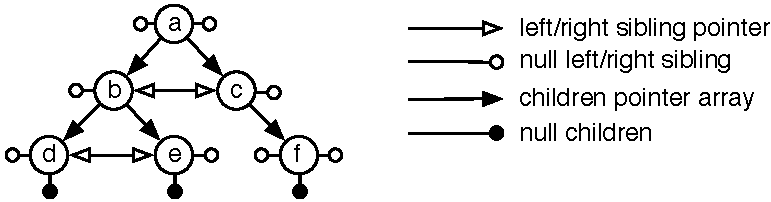
\includegraphics[width=0.6\columnwidth]{chapter6/treenaive}\label{subfig:pointer}} \linebreak
\subfloat[Compressed tree encoding]{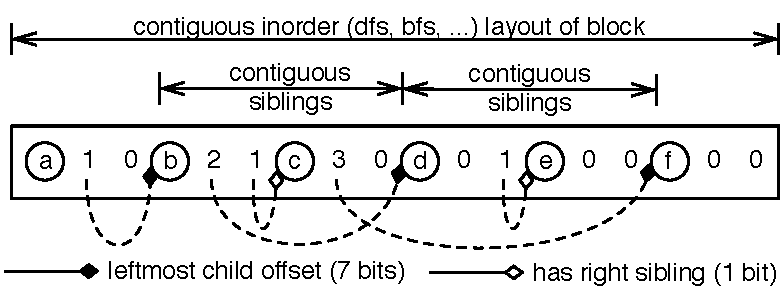
\includegraphics[width=0.6\columnwidth]{chapter6/treecompressed}\label{subfig:compressed}}
\caption{Two representations of the same tree: na\i{v}e pointer-based and optimized. The optimized version employs packing, breadth-first layout, and pointer compression via relative indexing.}
\label{fig:compression}
\end{figure}


\subsection{Data representation: Tuned and Compressed Tiles}

Our data representation optimizes for spatial and temporal locality and, as will be used by the scheduler, low overheads for operating over multiple nodes. Many researchers have proposed individual techniques for similar needs, and it is unclear which to use for what hardware. For example, mobile devices typically have smaller caches than laptops, they should exchange time for space. Our solution was to implement many techniques and build an autotuner~[[CITE]] that automatically choose an effective combination.  

Our autotuner runs sample data on multiple configurations for a particular platform to decide which configuration to use. The most prominent options are:

\begin{itemize}
\item C++ collections or contiguous arrays
\item tiling~\cite{tiling} of subtrees
\item depth-first or breadth-first ordering of nodes in a tile (with matching traversal order~\cite{Chilimbi:1999})
\item aligned data, or unaligned but more packed data
\item pointer compression
\end{itemize}
Several of the techniques are parameterized, so our tuner performs a brute force search for parameter values such as the maximum size of a subtree tile. To make the search tractable, we prune by manually providing heuristics, such as for parameter ranges.

The individual optimizations target several objectives:

\begin{itemize}
\item \textbf{Compression} Compressing the tree better utilizes memory bandwidth and decreases the working set size. We use two basic techniques: structure packing and pointer compression. Packing combines several fields in the same word of memory, such as storing 32 boolean attributes in one 32bit integer field. Similar to \citeauthor{compression}~\cite{compression}, compression encodes node references as relative offsets (16--20bits) rather than 32bit of 64bit pointers. Likewise,  as there are typically few siblings, instead of a counter of number of children (or siblings), we use an \code{isLastSibling} bit. Figure~\ref{fig:compression} depicts a tree using pointers and one of our representations: in the example, the compressed form uses 96\% fewer bits on a 64-bit architecture.

\item \textbf{Temporal and Spatial Locality}  The above compression optimizations improve locality by decreasing the distance between data. To further improve locality, we support rearranging the data in several ways .

Tiling~\cite{tiling} cuts the tree into subtrees and collocates nodes of the same subtree. It improves spatial locality because a node only reads and writes to its neighbors. Likewise, we support breadth-first and depth-first node orderings within a subtree (and across subtrees). Such a representation matches the tree traversal order~\cite{Chilimbi:19999} and therefore improves temporal locality. 

\item \textbf{Prefetching} We supports several options for prefetching to avoid waiting on data reads.  First,  the data access patterns with the data layout, so hardware prefetchers might automatically predict and prefetch data. Second, our compiler can automatically insert explicit prefetch instructions as part of the traversal. Finally, runahead processing~\cite{runaheadprocessing} pre-executes data access instructions. A helper thread traverses a subtree ahead of a corresponding evaluator thread, requesting node data while the evaluator is still computing an earlier thread. We only saw benefits of the first in practice, but leave the others as tunable.


\item \textbf{Parallel scheduling.} Reasoning about individual nodes, such as for load balancing and synchronization, leads to high overheads. By scheduling tiles rather than nodes, we cut overheads. Nodes correspond to tasks in our system, so our approach is a form of \emph{coarsening}. Furthermore, different synchronization strategies are possible for tiles, such as whether to use spin locks, so we autotune over the implementation options. 

We also support several scheduling options. First, we support third-party task schedulers, including Intel TBB~[[CITE]], Cilk~[[CITE]], and those of TesselationOS~[[CITE]]. Second, we built our own that uses a variant of work-stealing threads pinned to processors. It includes options such as whether to use hyper threads or not, and as we saw low speedups when using multiple sockets, how many threads to  use. Our autotuner picks between scheduler implementations.

\end{itemize}

Figure~\ref{fig:compression} depicts several of the data representation optimizations: packing, pointer compression, and a breadth-first layout. 




\begin{figure}
\centering
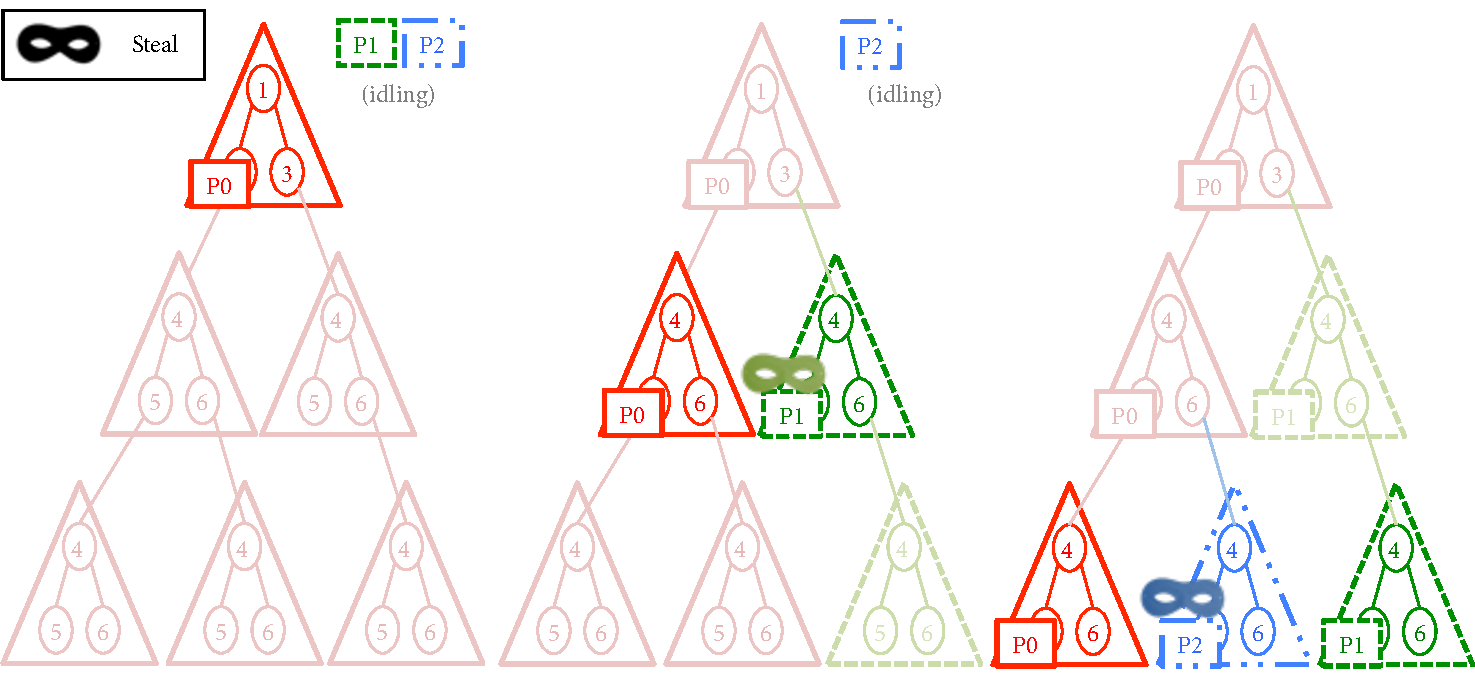
\includegraphics[width=1.0\columnwidth]{chapter6/wssimulation}
\caption{\textbf{Simulation of work stealing.} Top-down simulated tree traversal of a tiled tree by three processors in three steps.}
\label{fig:wssimulation}
\end{figure}


\begin{figure}
\centering
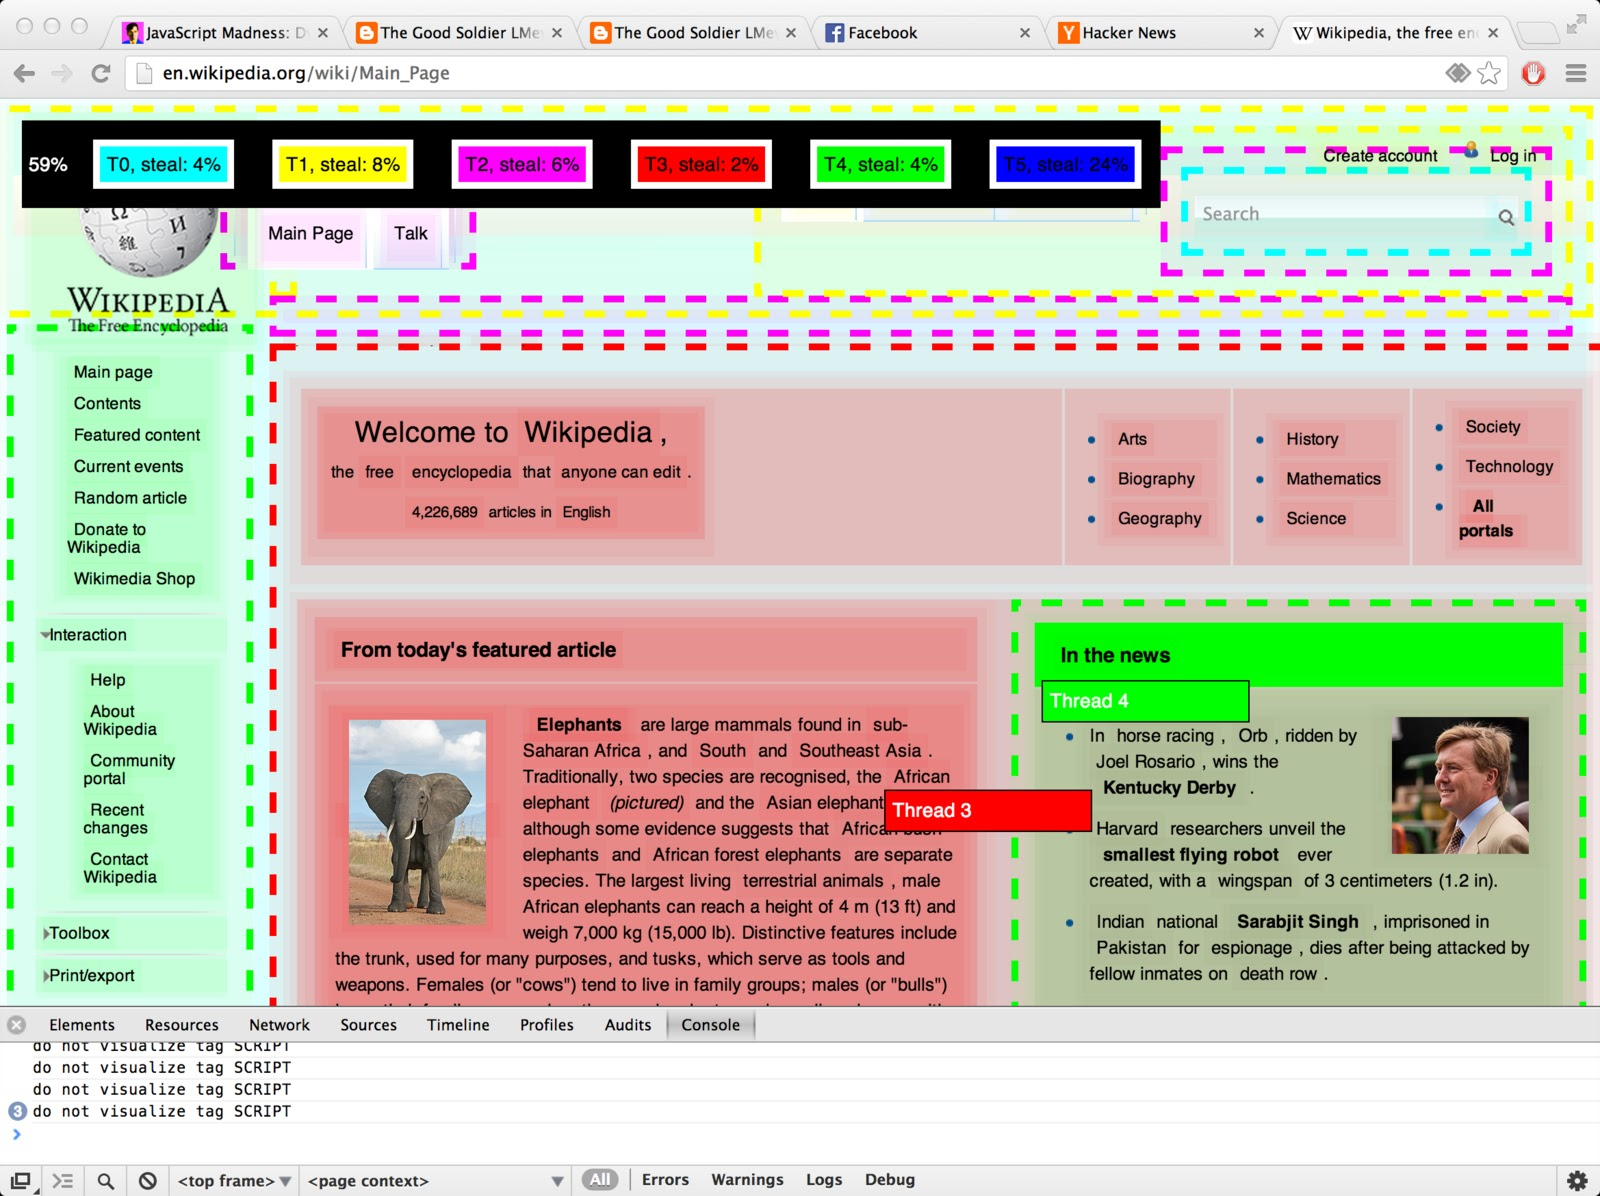
\includegraphics[width=1.0\columnwidth]{chapter6/workstealviz}
\caption{\textbf{Simulation of work stealing on Wikipedia.} Colors depict claiming processor and dotted boundaries indict subtree steals. Top-left boxes measure hit rate for individual processor.}
\label{fig:wswikipedia}
\end{figure}



\begin{figure}
\centering
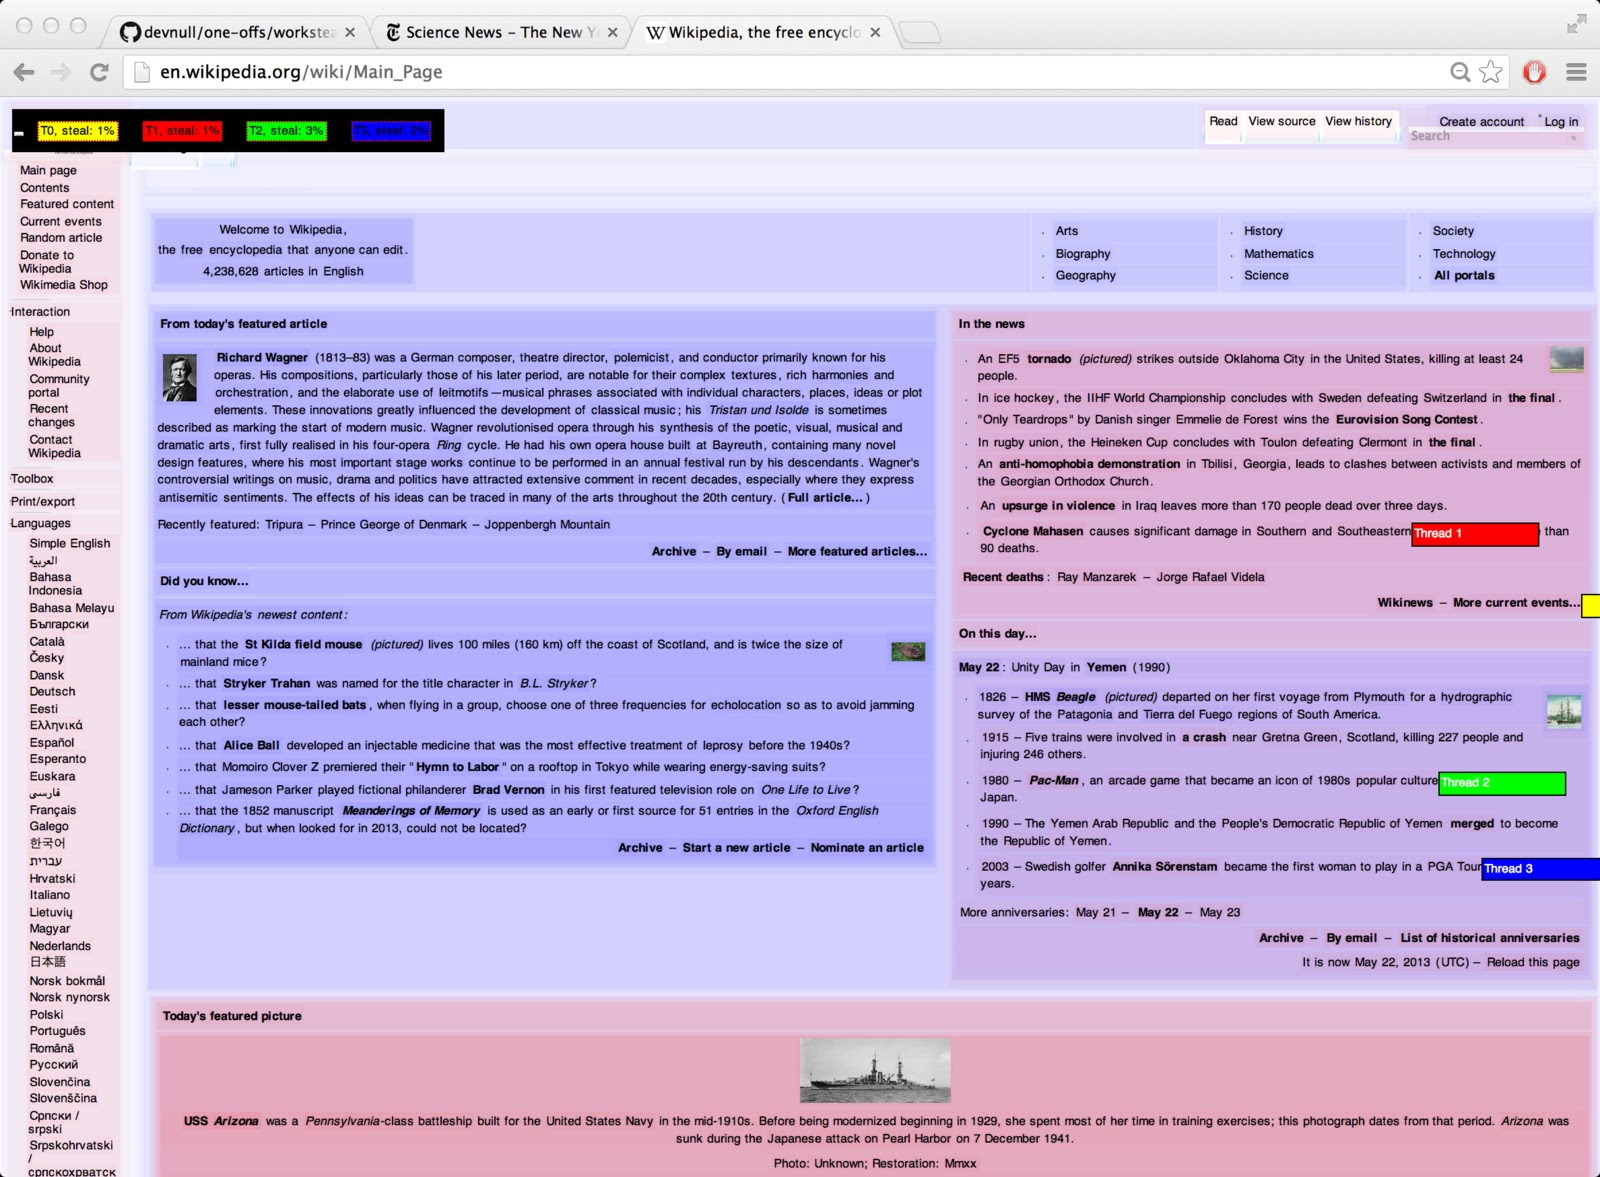
\includegraphics[width=1.0\columnwidth]{chapter6/workstealdelta}
\caption{\textbf{Temporal cache misses for simulated work stealing over multiple traversals.} Simulation of 4 threads on Wikipedia. Blue shade represents a hit and red a miss. 67\% of the nodes were misses. Top-left boxes measure hit rate for individual processor.}
\label{fig:wswikipediadelta}
\end{figure}

\begin{figure}
\centering
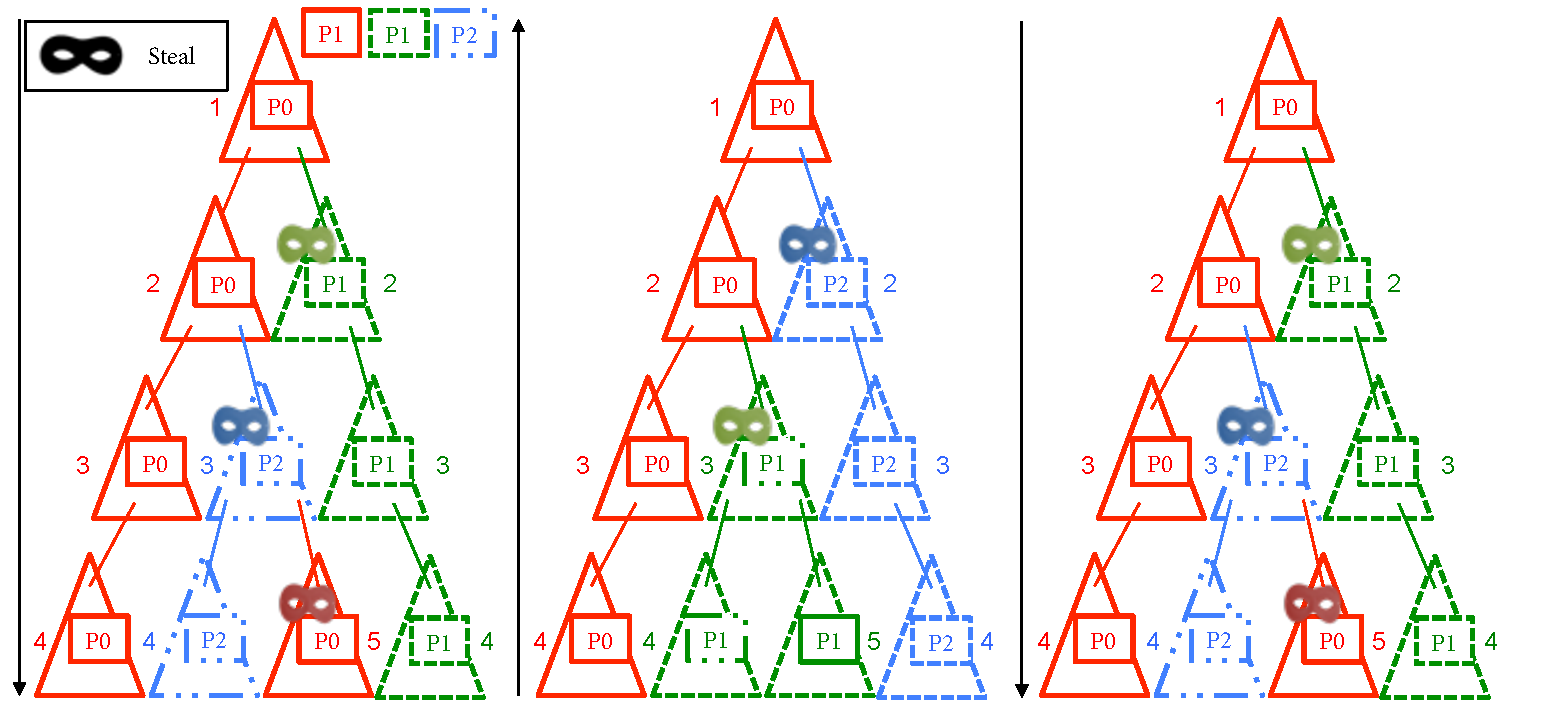
\includegraphics[width=1.0\columnwidth]{chapter6/wsbad}
\caption{\textbf{Dynamic work stealing for three traversals.} Tiles are claimed by different processors in different traversals.}
\label{fig:wsbad}
\end{figure}

\begin{figure}
\centering
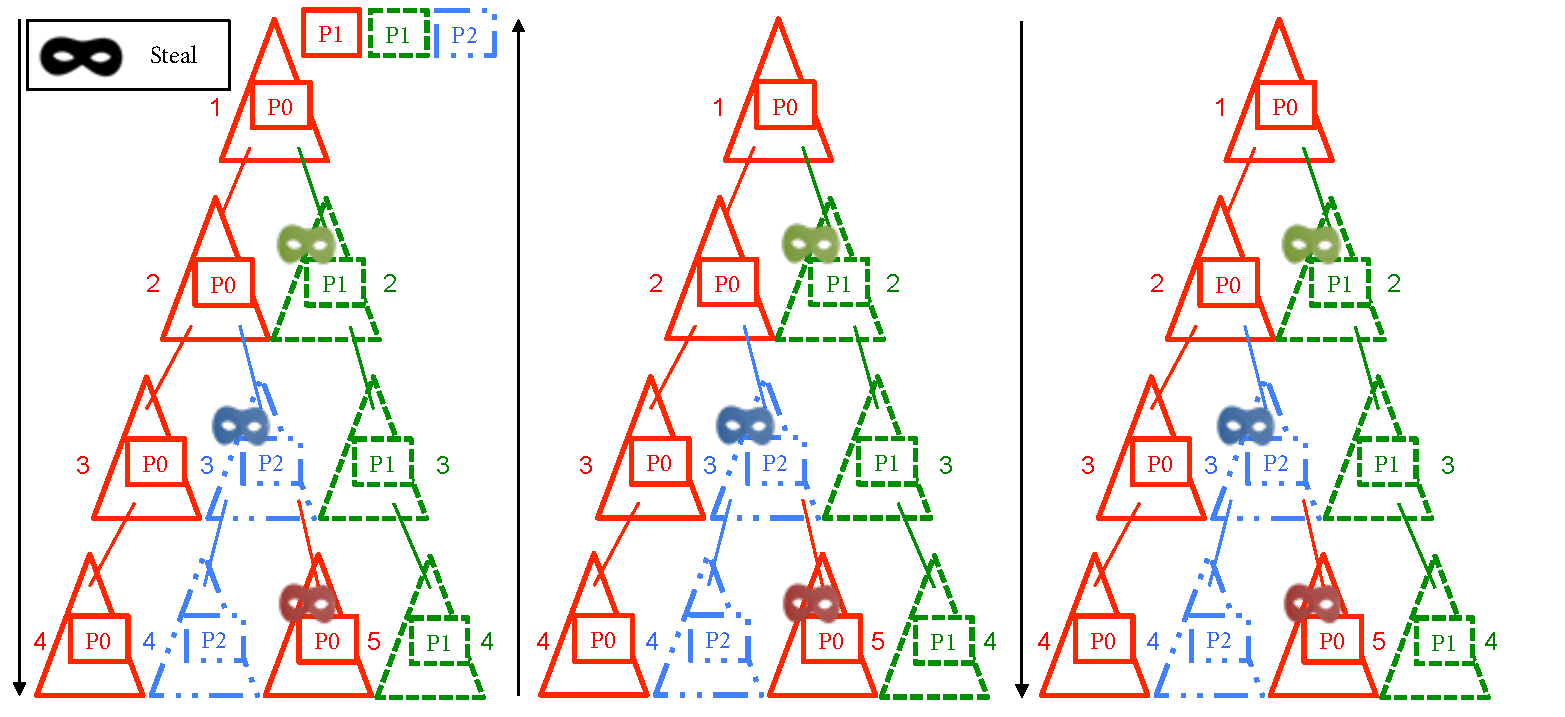
\includegraphics[width=1.0\columnwidth]{chapter6/wsgood}
\caption{\textbf{Semi-static work stealing.} Dynamic schedule for first traversal is reused for subsequent ones.}
\label{fig:wsgood}
\end{figure}


\subsection{Scheduling: Semi-static Work Stealing}
We optimize our tree traversal task scheduler for low overheads, high temporal and spatial data locality, and load balancing. Webpages are relatively small and use many traversals, so we found that aggressively optimizing individual traversals to be an important implementation concern. Our approach is to combine static scheduling~[[CITE]] with dynamic work stealing. We semi-statically schedule a traversal over the tree to as soon as it is available and reuse that schedule across traversals: this optimizes for temporal locality and low over-heads. We use work stealing as a heuristic for computing the first tree traversal for approximate load balancing.  We did not see significant speedups with the base approaches on their own, but our combination led to 7X parallel speedups. 


Our algorithm schedules the first traversal using work stealing~[[CITE]]. Work stealing was introduced as a dynamic scheduling algorithm that provides load balancing and spatial locality. Figure~\ref{fig:wssimulation} depicts a trace of three processors performing work stealing. Each processor operates on an internal task queue, and whenever a processor exhausts its internal queue, it will \emph{steal} from another processor's queue. In the case of a top-down tree traversal, acting upon an internal queue corresponds to a depth-first traversal of a subtree, and stealing corresponds to transferring ownership of an untraversed subtree. We lower overheads on the first traversal in two ways: we perform task coarsening by scheduling tiles rather than individual nodes, and we simulate the work stealing in one thread on a localized copy of the tiling meta data. The colors of Figure~\ref{fig:wswikipedia} show how different processors claim different nodes of a webpage during a parallel traversal: the localization of colors demonstrates the spatial locality of work stealing. Likewise, figure demonstrates that there are relatively few scheduling overheads (steals are indicated by dotted borders).

Work stealing suffers from runtime overheads and lack of temporal locality. To estimate the overhead, we simulated work stealing for 6 processors on Wikipedia. Assuming uniform compute time per node, 5\% of the nodes would trigger stealing. This cost is in addition to constant overhead to processing the internal per-processor task queues. The issue with temporal locality is that a node will be assigned to different processors across multiple traversals. Figure~\ref{fig:wswikipediadelta} shows which nodes must move across processors in a simulation 4 processors performing a sequence of  two traversals. 67\% of the nodes are red, indicating substantial movement. Both the steal rate and temporal miss rate worsen as the number of processors increase.

We use work stealing as a heuristic for semi-static scheduling so that the strengths of one address the weaknesses of the other. Semi-static scheduling precomputes the traversal order for each processor, which eliminates runtime overheads. Computing a load-balanced schedule can be quite expensive, however, because optimality is NP~[[CITE]]. Instead, we use work stealing as a heuristic by running a simulation in which the cost of each tile is the number of nodes in it and penalizing simulated steals. The trace through the simulation for a top-down traversal is used as the schedule for top-down traversals, and the reverse for bottom-up. Computing the schedule is fast -- a linear traversal over the tile meta data. 

Our approach achieves low overheads, high temporal and spatial locality locality, and load balanced evaluation. Temporal locality is enforced by reusing the same schedule across the traversals, and semi-static scheduling with a fast heuristic provides low overheads. Our work stealing heuristic provides spatial locality and an approximate form of load balancing.


\subsection{Evaluation}
